%----------------------------------------------------------------------------
\chapter{\bevezetes}
%----------------------------------------------------------------------------

Napjaink egyik fontos problémája a robotok társadalomban elfoglalt szerepének jövőbeni alakulása. A robot szó egyik (igen tág) értelmezése olyan gép, mely automatikusan komplex\todo[color=green]{mi az az automatikus komplex?:)} feladatok ellátására képes. Ezt alapul véve a számítási kapacitás és újonnan a mesterséges intelligencia gyors fejlődésének köszönhetően számos új területen jelentek, jelennek és jelenhetnek meg. Az iparban régóta \todo{mióta?} alkalmaznak robotokat. Ezek többnyire specifikus, jól behatárolt gyártási lépésekek végeznek. Bár emberi szemszögből az ellátott feladatok nehéznek tűnhetnek pontossági igényeik, nagy ismétlésszámuk és esetleg akár az adott feladat egyes lépéseinek számát tekintve is, programozói szempontból többnyire jól behatároltak. Egy másik terület, melyen jelentős segítség és előrelépés a robotok megjelenése a katasztrófaelhárítás és mentőakciók végrehajtása. \todo{Fukushima és hasonló esetek átnézése} Az emberek számára toxikus vagy nehezen hozzáférhető területek átvizsgálására illetve az ezen területeken történő munkavégzésre nagy előrelépést jelenthet robotok alkalmazása. \todo{cikket keresni ehhez}.

Bár a szociális és a szolgáltatóipari területeken alkalmazható robotok ötlete és kutatása nem új, a hétköznapi életben manapság mégis ritkán találkozhatunk robotokkal. Az 1980-as években például nagyvállalati kereskedelmi területeken már terjedni kezdtek takarítórobotok és néhány primitívebb otthon környezetbe szánt robot is \cite{engelberger_robotics_1989}, azonban utóbbiak gyenge funkcionalitásuk miatt nem terjedtek el. A háztartásban alkalmazható robotizált porszívók fejlesztése az 1990-es években nagy népszerűségnek örvendett \cite{brittain_autonomous_1993} \cite{brutzman_beyond_1993} \cite{coombs_robovac_1993}. Az ezredfordulóra a téma extenzív irodalommal rendelkezett \cite{fiorini_cleaning_2000}. A világ első kereskedelmi forgalomban is kapható robotporszívója az Electrolux Trilobite névre keresztelt terméke, melynek első prototípusa már 1996-ban bemutatásra került.
\todo{BBC-n mutatták be, amúgy az ilyet hogyan kéne hivatkozni?}
\todo[color=green]{misc, vagy ha van onlinevide, URL}
Mégsem jelenthetjük ki, hogy napjainkra elterjedtek lennének ezen, egy sok ember számára teherként felfogott feladatot megkönnyítő szerkezetek. Ennek két oka lehet a magas költség és az otthoni szokásokból adódó környezeti adottságokhoz való alkalmazkodóképtelenség. Nem érdemes drága robotba fektetni, ha a lakás felépítése vagy a különböző akadályok (pl. szétszórt ruhák, játékok) miatt szuboptimális eredményt kapunk, melyet utána az eredetihez mérhető időbefektetéssel szükséges kijavítanunk.

A háztartások előtt érdemes lehet a szolgáltatóipartban feladatokat ellátó robotok fejlesztésével foglalkozni. Például 2010-ben irodai környezetben takarító robotokkal már jobb tisztaságot lehetett elérni némi költségemelkedés mellett.\todo[color=green]{hivatkozás!!!} Egy irodai környezet, iskola vagy egészségügyi létesítmény lényegesen rendezettebb és kontrolláltabb környezetet nyújt. Jó alapot nyújthat továbbá a szociális robotika kutatásában a vendéglátóipari megoldások fejlesztése, mely szektor az emberekkel való interakciós helyzetek biztosításán túl a pandémia óta rekord munkaerőhiányban szenved, így újonnan felerősödött piaci rést is jelenthet.
\todo{Ezt újságcikkekkel lehetne behivatkozni, azt hogyan kéne?}

Vegyünk például egy éttermi pincér robotot. Az ilyen célú szerkezet megalkotására való törekvés az ókorig visszavezethető. Az első robotok között emlegetett, Philón által leírt Automate Therapaenis egy élethű méretű szobor volt, mely az egyik kezében tartott kancsóból bort töltött amennyiben másik kezébe poharat helyeztek (\ref{fig:automaid_philon}. ábra). Bár ma ezt inkább neveznénk trükkös italautomatának, mint robotnak, hasonló szándék állt mögötte. A mesterséges intelligenciabeli\todo[color=green]{ha van időd, akkor azért az ilyen nyakatekert fogalmazásokat érdemes átnézni (meg szvsz nem is helyes az írásmód de azt nem tudom biztosan)} és hardveres korlátok miatt a magas szintű, személyre szabott felszolgálói szolgáltatások kiváltása ma még nem lehetséges.
\todo{ezt jobban kifejteni?}
Ellenben több helyen jelentek meg az emberi kapcsolatoktól elszigeteltebb megoldások, például a futószalagos kiszolgálás vagy tableten történő rendelés az asztaltól. Emellett több helyen a magas szintű kiszolgálás helyett a személyzet hiánya vagy költséghatékonyság szempontjábóll inkább csak kiadószemélyzetet alkalmaznak. Ilyen esetekben hasznos lehet robotokat alkalmazni a munkaerő kiegészítése és/vagy a szolgáltatás színvonalának növelése céljából.

\begin{figure}[h]
    \centering
    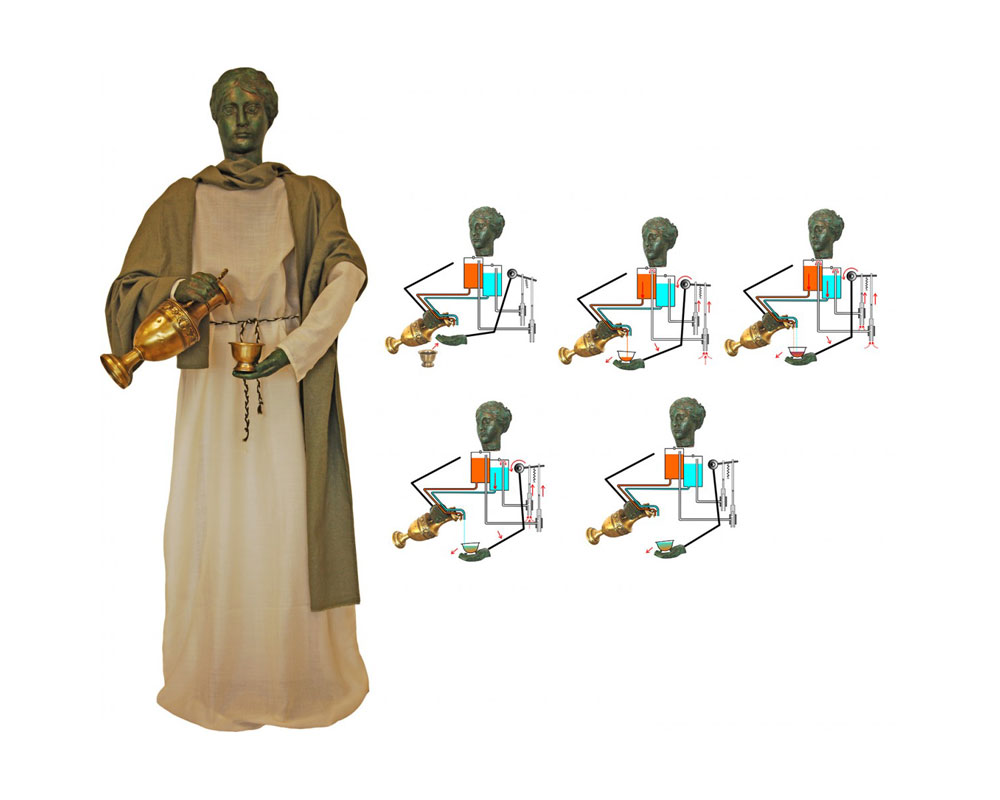
\includegraphics[width=\linewidth]{figures/automaid_philon.jpg}
    \caption{Philón automatája}
    \label{fig:automaid_philon}
\end{figure}

Az elmúlt évtizedekben növekvő figyelem irányult az emberek számára befogadható társrobotok kutatásának irányába. Sokan igyekeztek ezek közül humanoid alakkal rendelkező és humán pszichológián alapuló viselkedési mintázatokat utánozni próbáló megoldásokkal. Több kutatás is született antropomorf, érzelmeket kifejezni képes mesterséges fejek kialakításával kapcsolatban és bizonyított, hogy az emberek képesek felismerni az ezek által kifejezni kívánt érzelmeket \cite{lutkebohle_bielefeld_2010} \cite{delaunay_towards_2009} \cite{nitsch_emotions_2014}.\todo[color=green]{én nem tudom ez a template miért ilyen, de a számozott hivatkozásokat a megjelenésük sorrendjében szoktunk hivatkozni} Bár bizonyították, hogy az ezek alapján kiváltott érzelmek hasonló érzelmeket váltanak ki a valódi emberi arcok és kifejezések látványa által kiváltott érzelmekhez Chaminade és munkatársai \cite{chaminade_brain_2010} kimuattták, hogy ezek szintje és bizonyos esetekben az aktivált területek eltérést mutatnak egymáshoz képest. Az emberi interakciók és kifejezések komplexitásának és emellett az emberi agy fejlett arcfelismerő képességének köszönhetően könnyen futhatunk a modellezés során olyan kis eltérésekbe akár viselkedési mintázatokat, akár fizikai felépítést illetően, melyek negatív érzelmeket válthatnak ki. Ez a mára jól ismert "uncanny valley" (borzongások völgye) \cite{mori_bukimi_1970}.

Hasznos első lépés lehet tehát az emberi külalak és viselkedési mintázatok természetes, de ma még aligha megvalósítható vágyát elengedve alternatívák után néznünk. Az élővilág felé fordítva figyelmünket több érdekes példát is találhatunk szociális berendezkedés, kinézet és viselkedési mintázatok szempontjából is. A háziasítás során több állatfaj integrálódott az emberi életbe nem csupán haszonállatként, hanem egyéb célokra is. Legnépszerűbb példa a kutya, mely vélhetően az első háziasított faj volt. Bár régen vadászati célokat szolgált, mára legtöbben társállatként tartanak kutyát. Nem meglepő, hogy a világ második robotikus kisállata, a Sony által gyártott AIBO is kutya formájában látott napvilágot és mára negyedik generációját éli.

Külalak szempontjából érdekes betekintést biztosíthat még a számítógépes grafika, játékok és filmek világa. A filmiparban a számítógépes grafika elterjedése előtt nagymértékben alkalmaztak animatronikus modelleket. Ez ugyan mára költségessége miatt vissaszorult,\todo[color=green]{majd egy helyesírásellenőrzőt is engedj rá} ám a mai napig jelen van. Az ágazat művészei a kezdetek óta foglalkoztak azzal, hogy olyan karaktereket alkossanak meg, melyek adott érzelmeket váltanak ki. Azon túl, hogy inspirációt meríthetünk az emberek által kedvelt vonásokat illetően, megfigyelhetünk sikeres non-humanoid robotalakokat is. Nyilván ezek jó része fizikailag nem megvalósítható, azonban bizonyos elemeik átemelhetőek lehetnek a valóságba.
\todo{ábra}

\begin{figure}
    \centering
    \begin{subfigure}[b]{0.45\linewidth}
        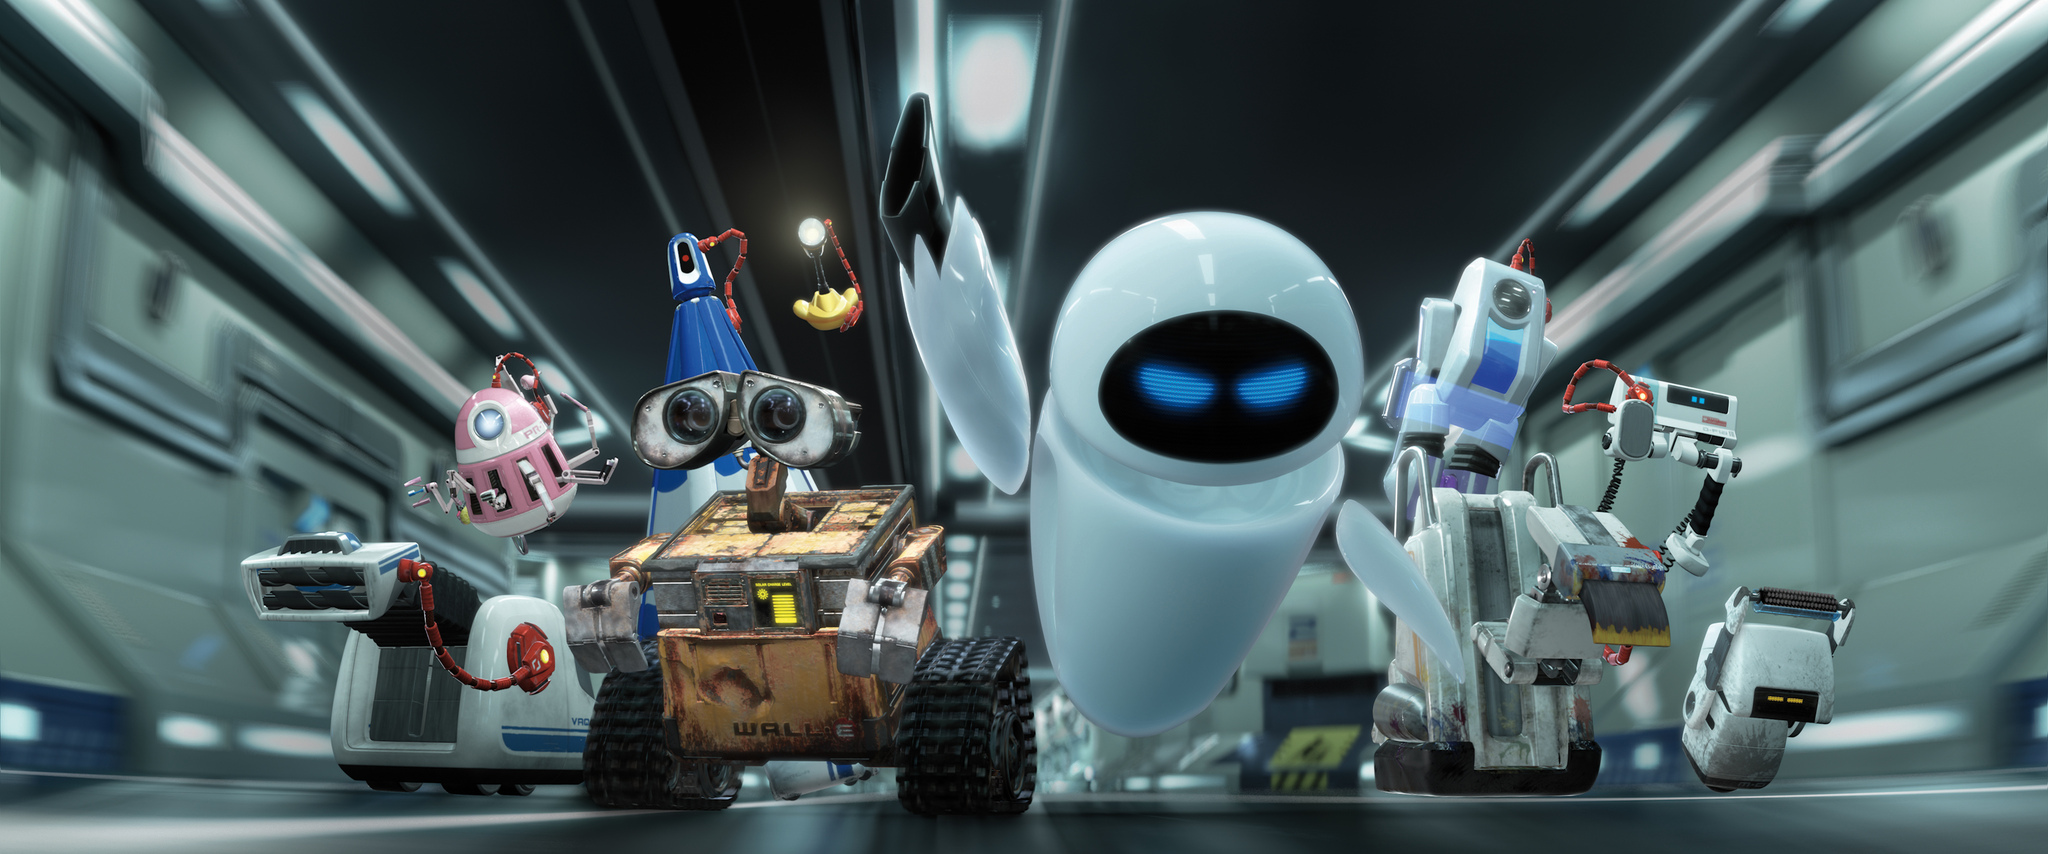
\includegraphics[height=3cm]{figures/non_humanoid_robots/wall_e.jpg}
    \end{subfigure}
    \begin{subfigure}[b]{0.15\linewidth}
        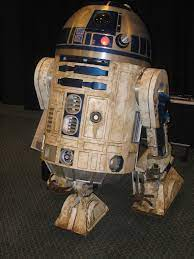
\includegraphics[height=3cm]{figures/non_humanoid_robots/r2d2.jpg}
    \end{subfigure}
    \caption{Példák non-humanoid robotokra filmekben.}
    \label{fig:neural_network_article_numbers}
\end{figure}

Fontos még, hogy a robotunk a befogadhatóságon túl feladata ellátására is képes legyen, hiszen végső soron valamilyen feladatkör elvégzésének céljából hozzuk létre. A felszolgálás feladata logisztikai és kommunikációs részekre osztható. Első lépésben a betérő látogatókat lokalizálnunk kell, majd ezt követően a rendelést valamilyen módon rögzítenünk kell. Ennek elkészülte után azt ki kell szállítanunk az asztalhoz, majd fogadnunk kell vendégeink fizetését a felszolgált tartalomért. A használt evőeszközöket ez után el kell szállítanunk bár vannak esetek, ahol ezt a vendég maga vagy külön személyzet végzi. A művelet során opcionálisan több ponton többlet kommunikációt végezhetünk a vendégekkel, de ez sem elsődleges cél. 

A navigációs és manipulációs feladatok a kereskedelmi- és gyártóipar automatizálásának köszönhetően mára megoldott feladatnak köszönhetőek. Bár az egyes cégek jellemzően nem hozzák nyilvánosságra drágán megalkotott kódbázisukat, a nyílt forráskód mozgalom népszerűségének köszönhetően mára elérhetővé váltak kedvünkre felhasználható és módosítható megoldások, melyek a fejlesztéshez szükséges időt nagymértékben csökkenthetik. Elérhetővé váltak továbbá olyan akár kereskedelmi forgalomban kapható megoldások is, melyek rugalmas alapot nyújthatnak specializáltabb kísérleti fejlesztéseknek. Ezek hozzáférhetőségét és számuk gyors növekedését segíti a Robot Operating System (Robot Operációs Rendszer, ROS) névre keresztelt szabad szoftverként fejlesztett projekt, mely nevével ellentétben nem operációs rendszerként, hanem inkább köztes kommunikációs rétegként szolgál. \todo[color=green]{pár hibát azért javítottam :)}

Hasonló gondolatok mentén és módon indult és folyik a Biscee névre keresztelt felszolgáló robot fejlesztése is az Eötvös Loránd Tudományegyetemen, mely projekthez diplomamunkám készítése során magam is becsatlakoztam. A robot alapját egy Robotnik\cite{noauthor_autonomous_nodate} RB-1 BASE mobil platform képzi, mely a(z)\todo[color=green]{majd ezeket azért nézd át hogy hova kell a, meg az}
\ref{fig:rb1_base}
. ábrán látható.
\begin{figure}
    \centering
    \begin{subfigure}[b]{0.25\linewidth}
        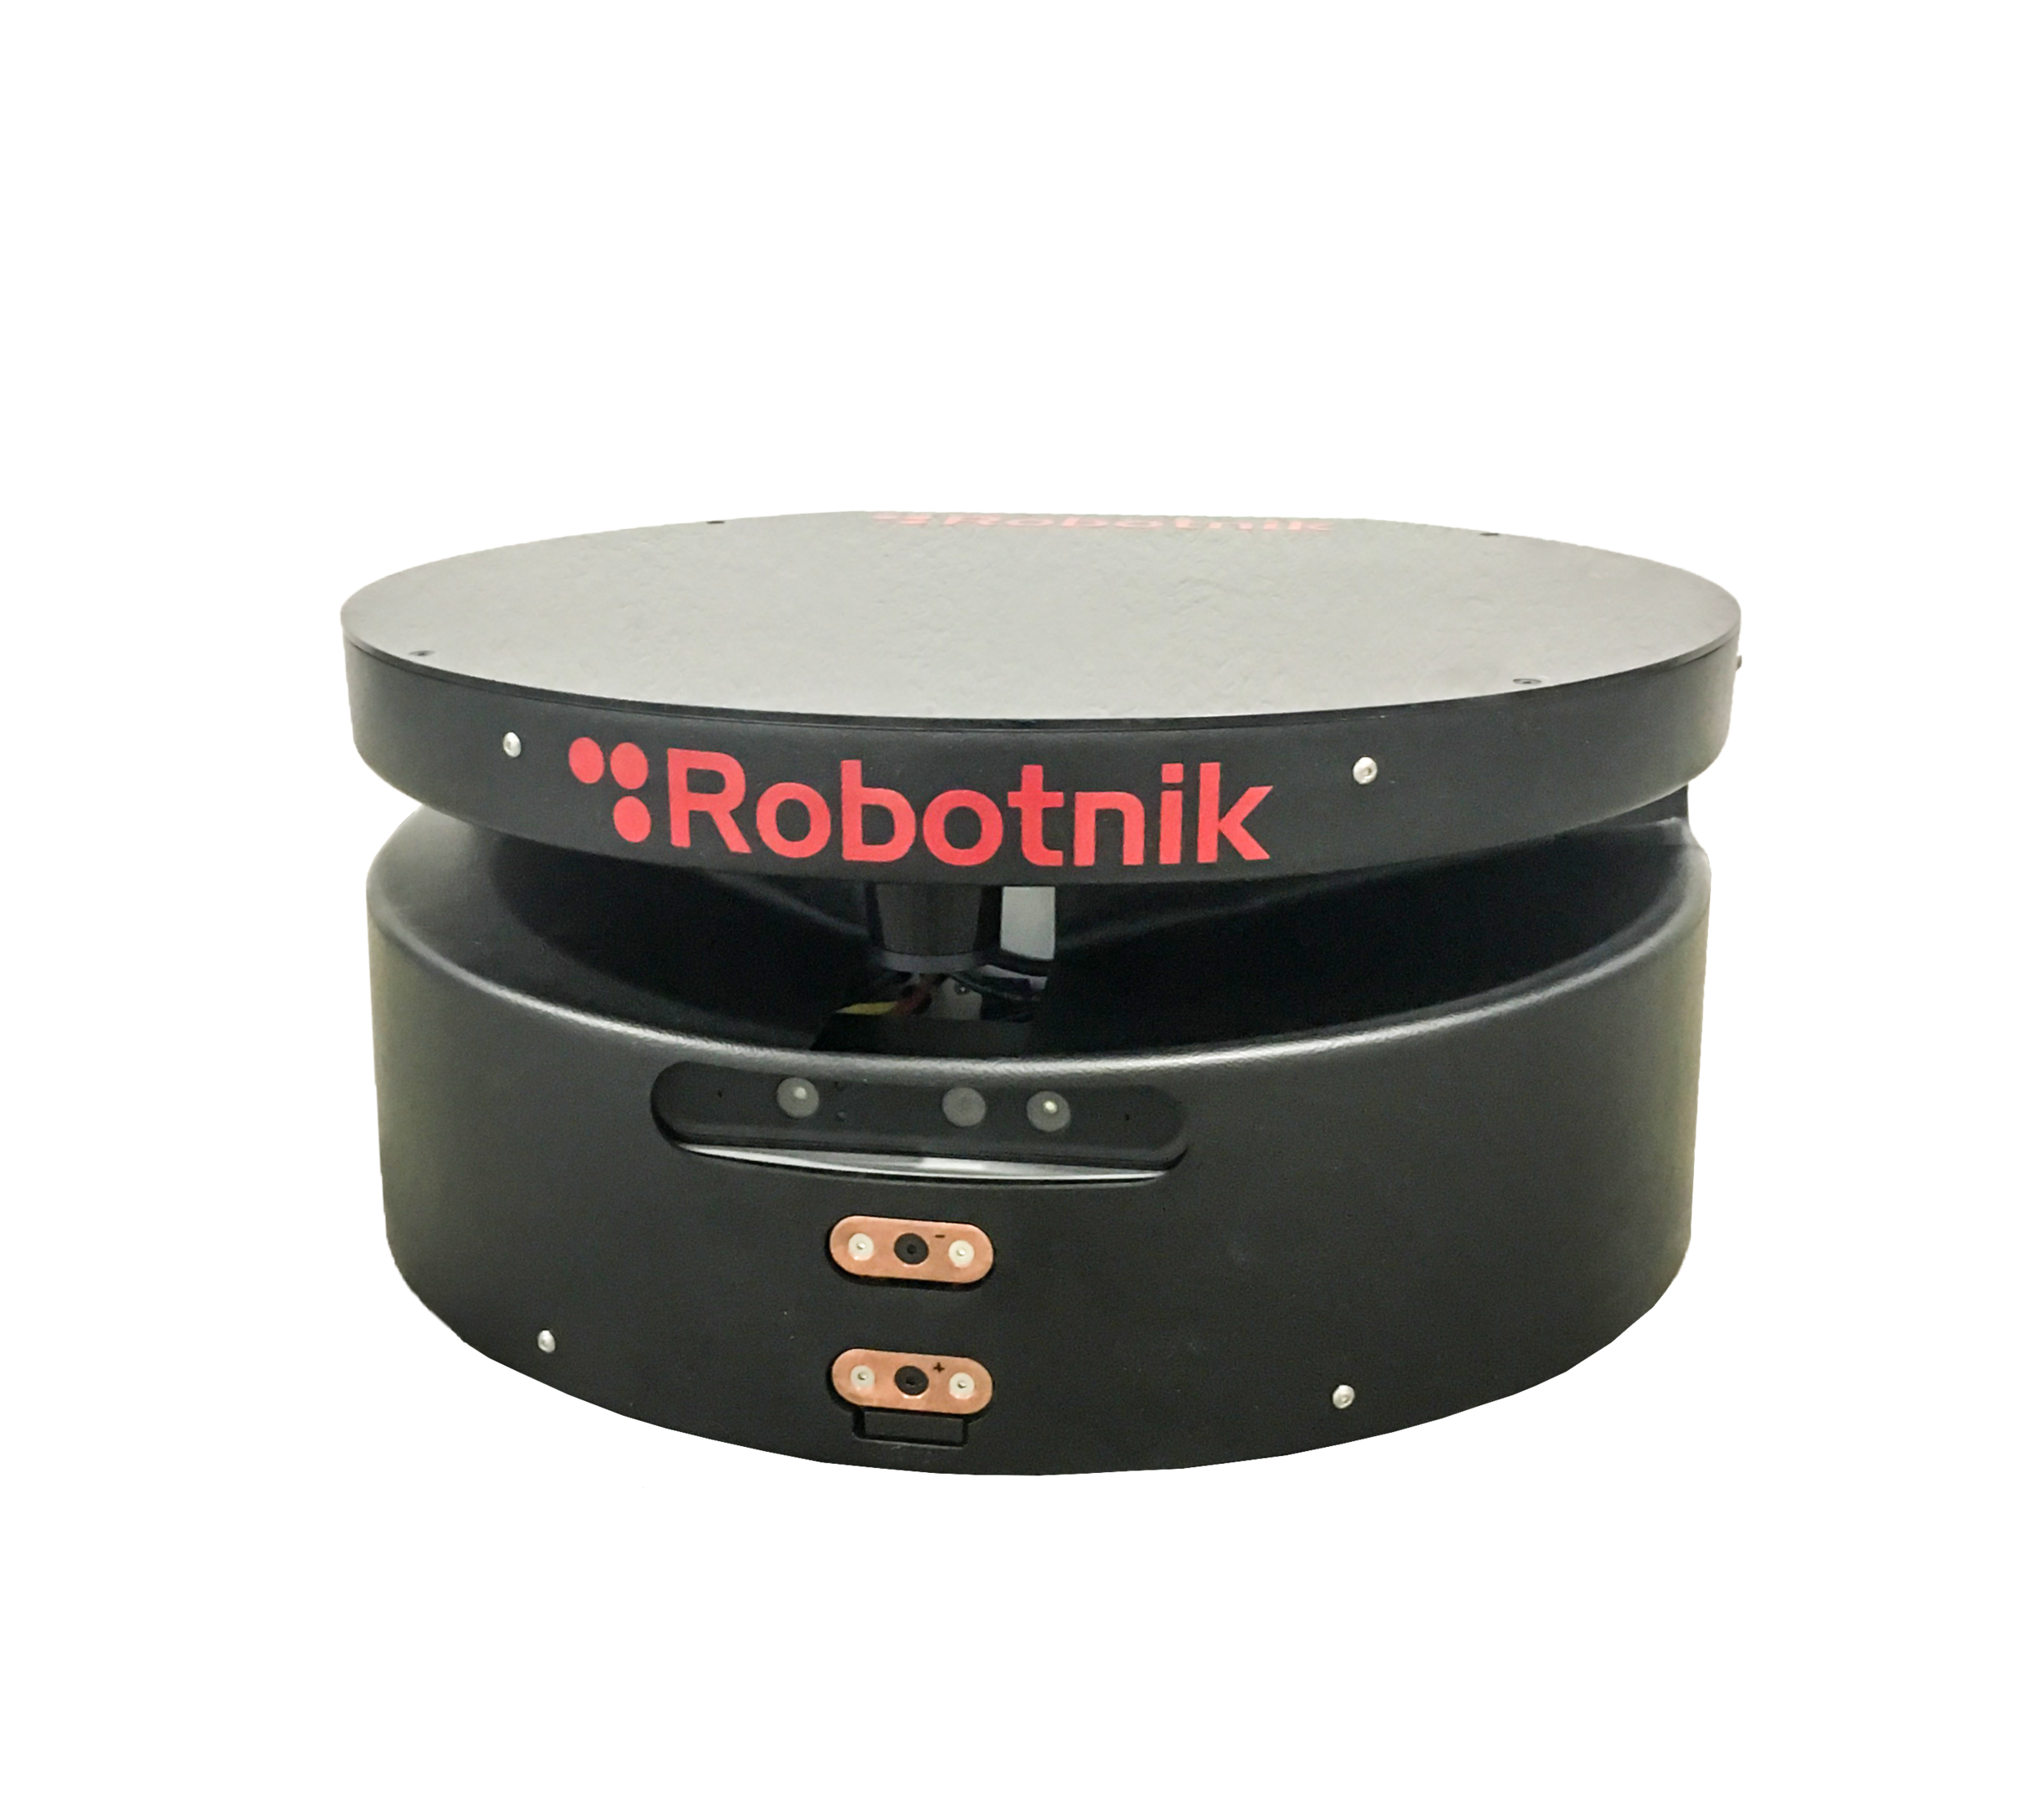
\includegraphics[width=\linewidth]{figures/Robotnik_RB-1-BASE-frontal.png}
        \caption{RB-1 BASE}
        \label{fig:rb1_base}
    \end{subfigure}
    \begin{subfigure}[b]{0.25\linewidth}
        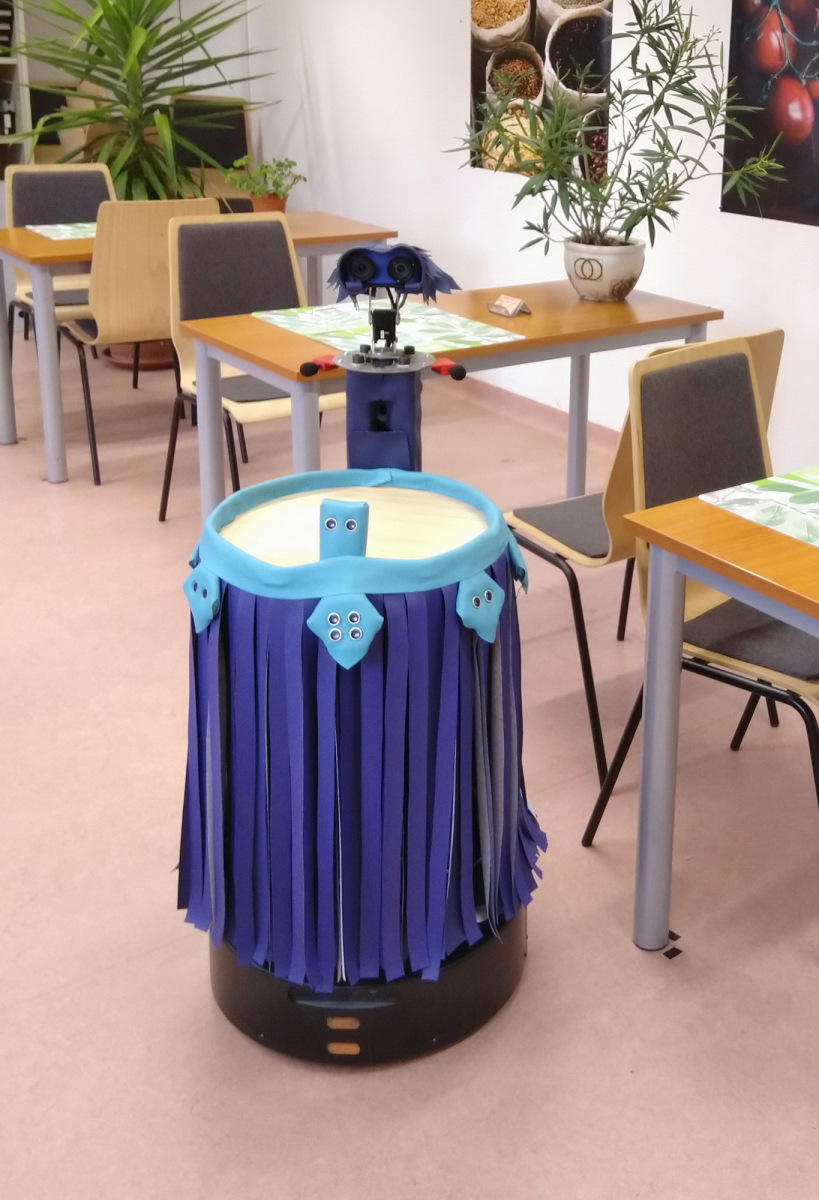
\includegraphics[width=\linewidth]{figures/biscee_frontal.jpg}
    \caption{biscee}
    \label{fig:biscee}
    \end{subfigure}
    \caption{Példák non-humanoid robotokra filmekben.}
    \label{fig:base_and_biscee}
\end{figure}
Erre bővítésképp egy felépítmény készült, melyen a kiszállítandó ételek elhelyezhetőek. A robot jelenleg ezek mozgatására alkalmas manipulátorral nem rendelkezik, a személyzetnek és a vendégeknek maguknak kell elhelyezni és elvenni a kívánt dolgokat. Az alap szenzorkészlet kiegészítésre került továbbá 8, navigációra és kommunikációra szolgáló ultrahang szenzorral és egy mozgatható fejrészen kialakított kamerára. Mivel az ember számára a szem páros szervként hat természetesen valójában két kamera is elhelyezésre került egymás mellett, azonban ebből jelenleg praktikus okokból csupán egy üzemel. Manapság jellemzően valamilyen polimer borítást alkalmaznak hasonló célú kísérleti robotoknál, ez azonban meglehetősen steril kinézetet okozhat. Biscee ehelyett műbőr borítást kapott, mely lényegesen kevésbé kelt mesterséges hatást. A megoldás emellett költséghatékony és a fejlesztés során rugalmasan alakítható és könnyű hozzáférést biztosít az alkatrészekhez és a kábelezéshez. A fent leírtak megfigyelhetőek a \ref{fig:biscee}.ábrán.

A munka során első lépésben másodlagos feladatként a bázisrobot szimulációját kiegészítettem a felépítmény extra szenzoraival és ROS nodejaival. A szimuláció futtatható mind virtuális környezetben mind konténerizálva, ily módon előzetes, biztonságos tesztelési lehetőséget biztosítva a robot mozgását és viselkedését fejlesztő munkatársaim számára. Elsődleges feladatom a roboton található kezdetleges arcfelismerő megoldás továbbfejlesztése volt. Ennek potenciális felhasználási lehetőségei sokrétűek, elsődleges kitűzött célja az előző gondolkodási vonalat követve a következő.

A kitűzött célfeladat alapvető szociális interakciót, kommunikációt igényel. Amennyiben ez nincs jelen a biztosított megoldás a magasan specializált, drága infrastruktúra kiváltásán túl nem nyújt lényegi előnyt például a futószalagos kiszolgálással szemben. Mindennapi életből származó intuitív tapasztalataink alapján kijelenthető, hogy kellemetlen, mikor egy vendéglátásra szakosodott létesítménybe betérve nem érezzük a kiszolgáló személyzet felénk irányuló figyelmét. Természetesen a túlságosan intruzív figyelem is negatív érzelmeket kelthet, azonban későbbi viselkedésbeli mintatervezési feladat. Fontos tehát, hogy a felszolgálási feladat előzetes lépéseként képesek legyünk kifejezni a vendég számára a felé irányuló figyelmet.

Az emberi kommunikáció egyik igen fontos nonverbális összetevője a szemkontaktus. Alkalmazása azonban nem korlátozódik ember-ember kapcsolatokra. Fő érzékszervként az állatvilágban is lényeges szerepet játszik, így kisállatainkkal folytatott interakcióink során is előszeretettel használjuk. Kutyáknál például az emberekhez hasonlóan megfigyelhető a szemlesütés és hasonló viselkedések, de helyzettől függetlenül is szeretünk állatokhoz tekintet és kinézet alapján hangulati tartalmat kapcsolni. A szemek emellett a verbális kommunikációt nem vagy csak korlátozottan alkalmazó képzeletbeli karakterek érzelemkifejezésében is fontos szerepet játszanak ezzel bizonyítva, hogy fontosságuk a való világ keretein is túlnyúlik. Ezekre látható néhány példa a
\todo{ábra}
.ábrán.
\begin{figure}
    \centering
    \begin{subfigure}[b]{0.24\linewidth}
        
\includegraphics[width=\linewidth]{figures/eye/grumpy_cat.jpg}
    \end{subfigure}
    \begin{subfigure}[b]{0.24\linewidth}
        
\includegraphics[width=\linewidth]{figures/eye/doge.jpg}
    \end{subfigure}
    \begin{subfigure}[b]{0.24\linewidth}
        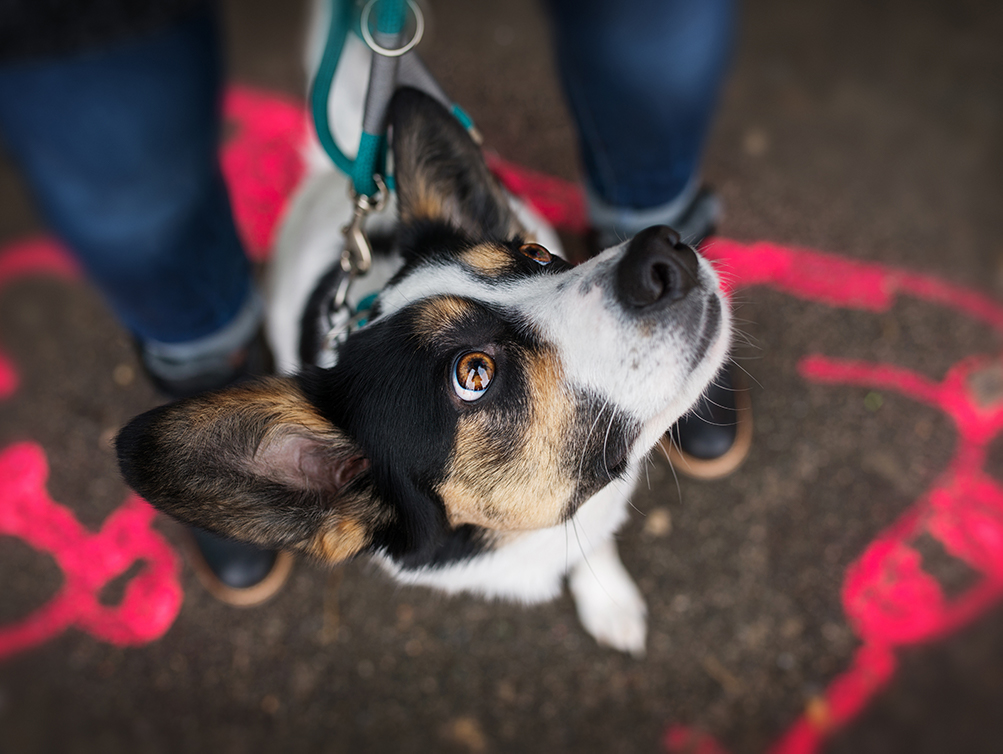
\includegraphics[width=\linewidth]{figures/eye/dog_attention.jpg}
    \end{subfigure}
    \begin{subfigure}[b]{0.24\linewidth}
        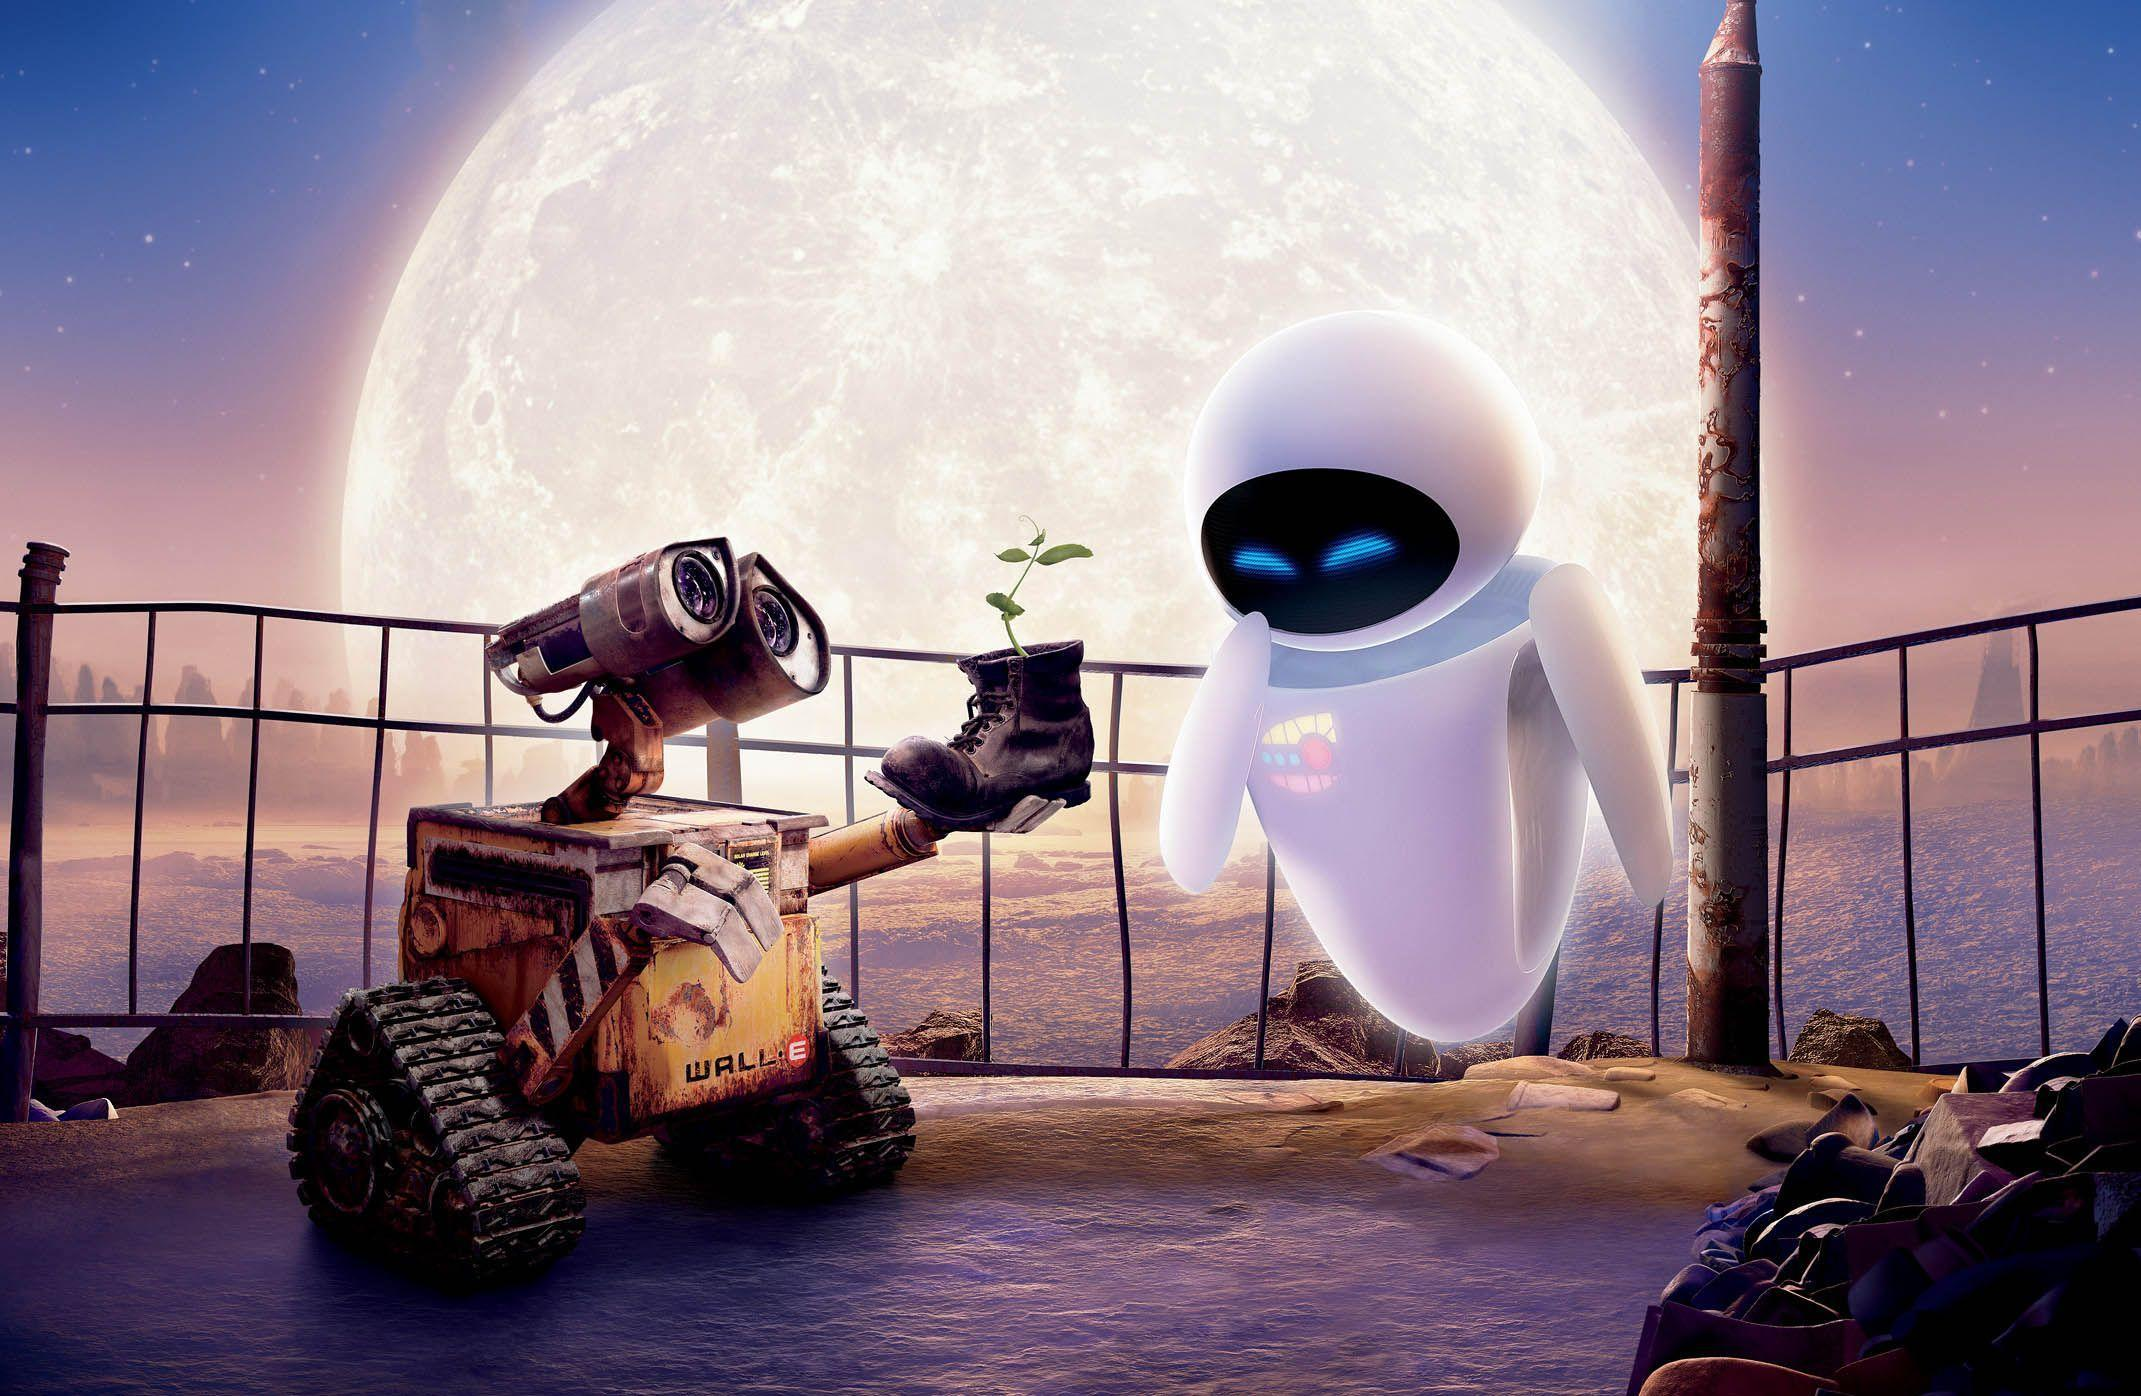
\includegraphics[width=\linewidth]{figures/eye/wp1816244.jpg}
    \end{subfigure}
    \caption{Példák non-humanoid robotokra filmekben.}
    \label{fig:eye_importance}
\end{figure}
A tekintet az adott személy felé irányítása, a szemkontaktus felvétele a kommunikációs csatorna megnyitásának szempontjából kulcsfontosságú nonverbális eszköz. Az első szempontjából elégséges, a második szempontjából pedig szükséges ehhez az alany arcának helyzetének ismerete. Ennél fogva szükségessé válik valamilyen szintű arcfelismerési módszer alkalmazása. Ennek szintjét és módját, az alkalmazott szenzorokat és algoritmusokat az adott helyzethez és limitációkhoz kell igazítani. Esetünkben a szenzorok és a hardver adottak: Biscee kamerái és az RB1-es platform hardvere. Adottak továbbá a roboton futó jelenlegi Ubuntu Linux operációs rendszer és ROS verzió. A roboton előzetesen futó kezdetleges megoldás a feladatot számosítás nélkül aránylag megfelelő pontossággal és 2 fps sebességgel képes ellátni. A cél ennek lehetőségekhez mért javítása volt.

Mivel a fejlesztőgárdában kapcsolódó területeken tapasztalt személy nem szerepelt, első lépésben a témában fontos alapvető fogalmak, illetve a jelenleg elterjedt megoldások gyakorlati és rövid elméleti megismerésével kezdtem. Ezt követően részletesebb irodalmi kutatást végeztem a létező arc- és objektumfelismerő eljárásokról és az ezeknél alkalmazott benchmark teljesítményértékelési lehetőségekkel kapcsolatban. Következő lépésben a létező algoritmusok körét leszűkítettem a célfeladatnak és hardveres limitációknak megfelelően, majd ezeket kiértékelve összehasonlítottam. A kiválasztott algoritmust a roboton futó ROS rendszerrel kompatibilis nodeban helyeztem el. A kutatás menetét és a kapott eredményeket a következő fejezetekben tárgyalom.
\todo{ide még lehetne írni pár mondatot az erőforrások optimalizálásáról (gnome kilövés, túlpörgő websocket node)}